%%%%%%%%%%%%%%%%%%%%%%%%%%%%%%%%%%%%%%%%%%%%%%%%%%%%%%%%%%%%%%%%%%%%%%%%%%%%%%%%
% TUM-Vorlage: Präsentation - Beispiele
%%%%%%%%%%%%%%%%%%%%%%%%%%%%%%%%%%%%%%%%%%%%%%%%%%%%%%%%%%%%%%%%%%%%%%%%%%%%%%%%


\begin{frame}
\frametitle{2 Dimensional Force Calculation}
	\begin{textblock}{0}(0,3.5)
	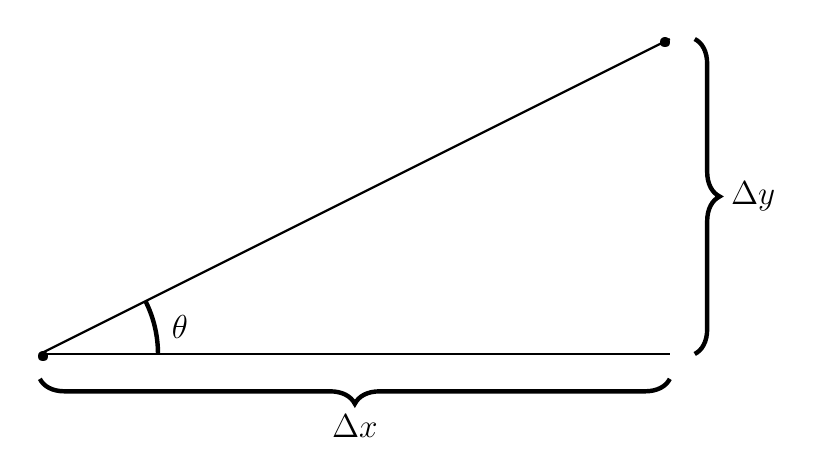
\begin{tikzpicture}[ultra thick]
	
	\foreach \Point in {(0.05,-0.05), (7.95,3.95)}{
		\node at \Point {\textbullet};
	}
	
	\draw[thick]	(0,0) -- (8,4);
	\draw[thick]    (0,0) -- (8,0);
	
	\draw (1.5,0) arc (0:atan(4/8)):1.5)
	node[pos = 0.5, right = 2pt]{\large $\theta$};
	
	\draw [decorate, decoration = {brace, raise = 9pt, amplitude = 9pt}] 	(8,0) --  (0,0)
	node [pos = 0.5, below = 18 pt]{\large $\Delta x$};
	\draw [decorate, decoration = {brace, raise = 9pt, amplitude = 9pt}] (8,4) --  (8, 0)
	node [pos = 0.5, right = 18 pt]{\large $\Delta y$};
	\end{tikzpicture}
	\end{textblock}
	
	\begin{textblock}{7}(6,4)
		\large
		\begin{equation}
			\Delta x = x_2 - x_1
		\end{equation}
		\begin{equation}
			\Delta y = y_2 - y_1
		\end{equation}
		\begin{equation}
			|F| = \frac{m_1 m_2}{\Delta x^2 + \Delta y^2}
		\end{equation}
		
	\end{textblock}´

	\begin{textblock}{10}(2, 10)
		\large
		\begin{equation}
			F_x = \cos(\theta) \cdot |F| = \Delta x \cdot \frac{m_1 m_2}{\left( \Delta x^2 + \Delta y^2 \right)^{3/2}}
		\end{equation}
		\begin{equation}
			F_y = \sin(\theta) \cdot |F| = \Delta y \cdot \frac{m_1 m_2}{\left( \Delta x^2 + \Delta y^2 \right)^{3/2}}
		\end{equation}
		
		
	\end{textblock}
	
\end{frame}

\begin{frame}[fragile]
	\frametitle{Utilizing $F_{ij} = -F_{ji}$}
	\large 
	The naive approach ($n\cdot (n-1)$ Force calculations):\\
	%\vspace{-0.1cm}
	\begin{Verbatim}
for all Particles p:
	for all Particles p'!=p:
		computeF(p,p')
	\end{Verbatim}
	\centering
	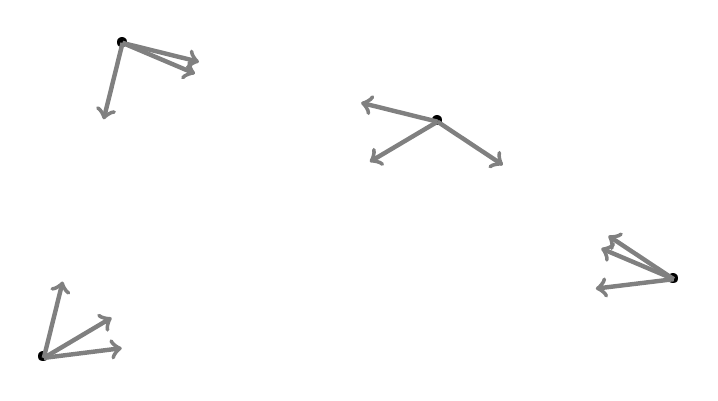
\begin{tikzpicture}[ultra thick]
		\foreach \Point in {(0,0), (1, 4), (5,3), (8,1)}{
			\node at \Point {\textbullet};
		}
		\visible<1>{
			\draw[->, gray]{(0,0) -- (0.24, 0.97)};
			\draw[->, gray]{(0,0) -- (0.86, 0.51)};
			\draw[->, gray]{(0,0) -- (0.99, 0.124)};
			%\draw[->, gray, scale=0.24]{(0,0) -- (1,4)};
			%\draw[->, gray, scale=0.17]{(0,0) -- (5,3)};
			%\draw[->, gray, scale=0.125]{(0,0) -- (8,1)};
		}
		
		\visible<2>{
			\draw[->, gray]{(1,4) -- (0.76, 3.03)};
			\draw[->, gray]{(1,4) -- (1.97, 3.76)};
			\draw[->, gray]{(1,4) -- (1.92, 3.61)};
		}
		\visible<3>{
			\draw[->, gray]{(5,3) -- (4.14, 2.49)};	
			\draw[->, gray]{(5,3) -- (4.03, 3.24)};	
			\draw[->, gray]{(5,3) -- (5.83, 2.45)};	
		}
	
		\visible<4>{
			\draw[->, gray]{(8,1) -- (7.01, 0.88)};	
			\draw[->, gray]{(8,1) -- (7.08, 1.39)};	
			\draw[->, gray]{(8,1) -- (7.17, 1.55)};	
		}
	%\begin{textblock}{7}(5,7)
	%	\large
	%	\visible<5>{$n\cdot(n-1) \text{computations of F necessary}$} hässlich aber sonst nimmt er es nicht
	%\end{textblock}
		
	\end{tikzpicture}
	\end{frame}
	
	\begin{frame}[fragile]
		\frametitle{Utilizing $F_{ij} = -F_{ji}$}
		\large 
		A better approach ($\frac{1}{2} n\cdot (n-1)$ Force calculations):\\
		\begin{Verbatim}
for all ParticlePairs (p,p'):
	computeF(p,p')
		\end{Verbatim}
	\centering
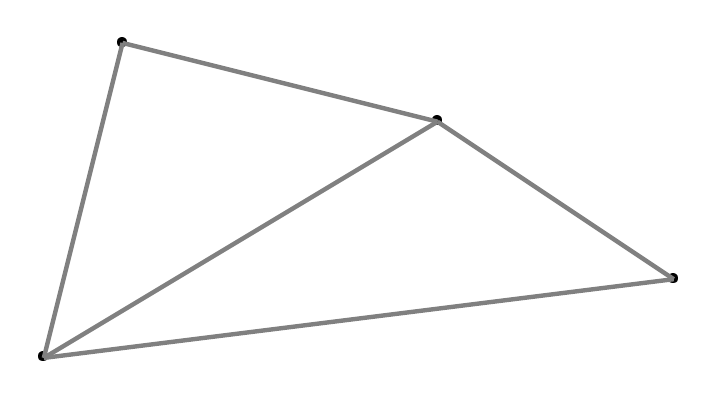
\begin{tikzpicture}[ultra thick]
\foreach \Point in {(0,0), (1, 4), (5,3), (8,1)}{
	\node at \Point {\textbullet};
}
\visible<1>{\draw[gray] (0,0) -- (1,4);}
\visible<2>{\draw[gray] (1,4) -- (5,3);}
\visible<3>{\draw[gray] (5,3) -- (8,1);}
\visible<4>{\draw[gray] (0,0) -- (5,3);}
\visible<5>{\draw[gray] (0,0) -- (8,1);}
\end{tikzpicture}
	
\end{frame}

%%%%%%%%%%%%%%%%%%%%%%%%%%%%%%%%%%%%%%%%%%%%%%%%%%%%%
%% Folie: Gültigkeit der Masterfolien              %%
%%%%%%%%%%%%%%%%%%%%%%%%%%%%%%%%%%%%%%%%%%%%%%%%%%%%%

\begin{frame}
\frametitle{Refactoring}
\vspace{-0.5cm}
´\begin{figure}
	\centering
	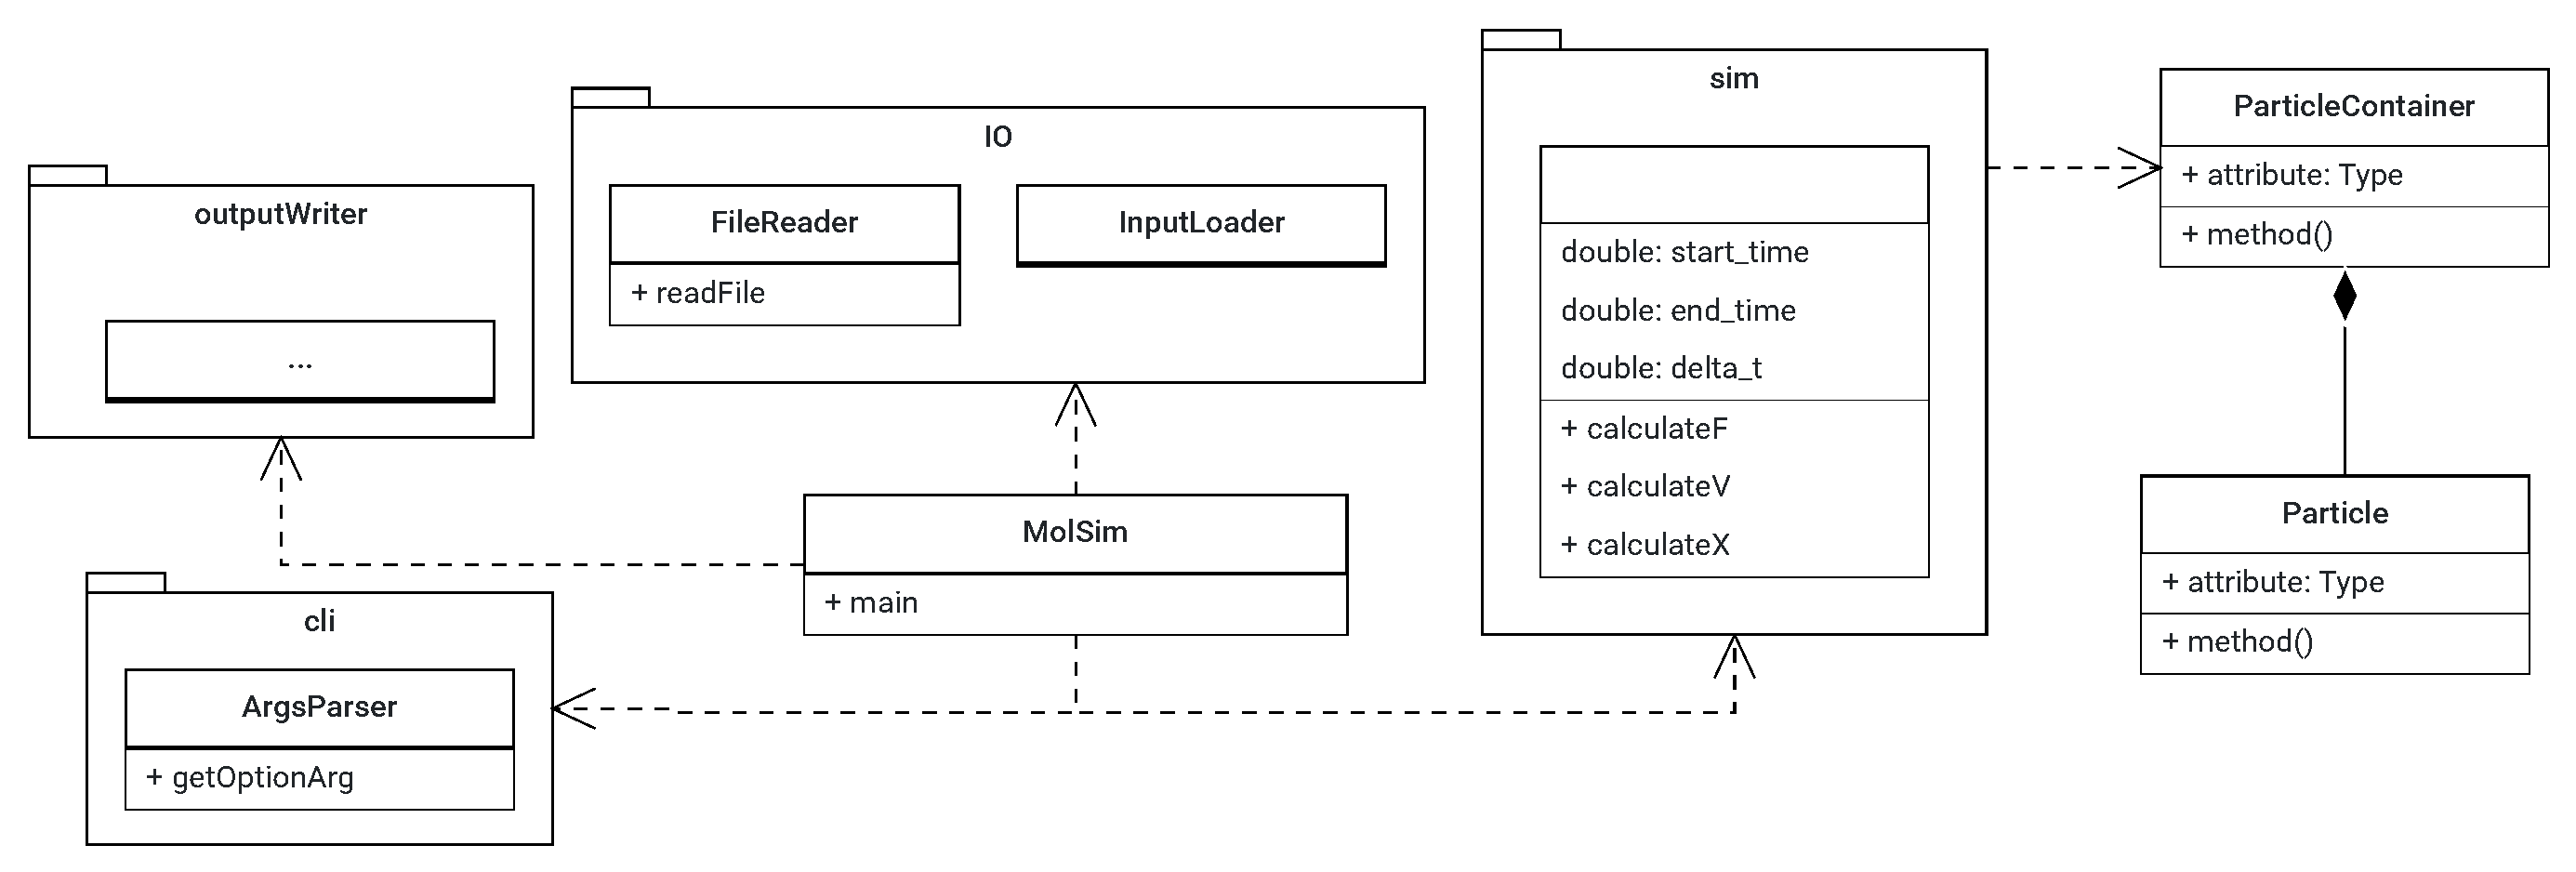
\includegraphics[height=0.5\textheight]{UMLClassDiagram-1}
	\label{fig:umlclassdiagram-1}
\end{figure}
\end{frame}

\begin{frame}[fragile]
	\frametitle{Use of the Program}
	\vspace{0.7cm}
	\begin{Verbatim}
❯ ./MolSim --help
Welcome to MolSim Help
Usage:
MolSim <input-files> <options>
Options:
--help, -h              Prints this screen.
-dt <value>             Sets delta time to <value>. If -dt is not specified default value is used.
-et <value>             Set end time to <value>. If -et is not specified default value is used.
-o <name>               Set base name of output files. DO NOT USE A PATH! Default is 'result'.
-of <path>              Set path to output folder. Default is ./output
	\end{Verbatim}
\end{frame}

\begin{frame}[fragile]
\frametitle{Generic IO}
\vspace{0.7cm}
\begin{lstlisting}[language=C++]
template <typename LOCATOR, void (*LOAD)(LOCATOR, std::list<Particle>&)>
class InputLoader {
	private:
	std::list<Particle> buffer;
	LOCATOR locator;
	public:
	explicit InputLoader(LOCATOR loc) : locator(loc) {}
	InputLoader(const InputLoader& i) = delete;
	void reload() { LOAD(locator, buffer); }
	void getParticles(std::vector<Particle>&buf) {...}
};
\end{lstlisting}
\end{frame}

\begin{frame}
    \frametitle{Refactoring surprises}
		\large
		\begin{itemize}
			\item<1-> Task: Verify the correctness of the program after major refactoring
			\item<2-> Idea: string-compare the new output with the old output. If the program works as intended it should be the same
			\item<3-> Observation: Very slight differences in the outputs generated (unoberservable in the videos)
		\end{itemize}
		\visible<4->{What happened:}
		\begin{itemize}
			\item<5-> floating point operations are not associative $\rightarrow$ both outputs were "`correct"'
			\item<6-> probably some compiler magic
			\item<7-> Funfact: Compiling the exact same code with the exact same compiler settings will result in the same output
			\item<8-> First-hand encounter of the inaccuracies of numerical programming
		\end{itemize}

\end{frame}
\clearpage

\begin{frame}
	\frametitle{bloopers}
	%TODO
\end{frame}

\begin{frame}
	\frametitle{Ideas, Roadblocks and Pain}
	\large
	\begin{itemize}
		\item<1-> Custom CSS Doxygen didn't cooperate
		\item<2-> Disproportion of time invested $\leftrightarrow$ relevance
		\item<3-> libxerces, Eigen deplo´yment pain
		\item<4-> Cmake, Doctest details
		\item<5-> Iterator-related debate
		\item<6-> Data structure locality (for later exercises)
	\end{itemize}
	
\end{frame}